\section*{Ejercicio 1.}

Para este punto escribimos el siguiente código.

\begin{Verbatim}[commandchars=\\\{\}]
\PY{k+kt}{void} \PY{n+nf}{TaskConsola}\PY{p}{(}\PY{k+kt}{int} \PY{n}{pid}\PY{p}{,} \PY{n}{vector}\PY{o}{\PYZlt{}}\PY{k+kt}{int}\PY{o}{\PYZgt{}} \PY{n}{params}\PY{p}{)} \PY{p}{\PYZob{}}
    \PY{k+kt}{size\PYZus{}t} \PY{n}{n} \PY{o}{=} \PY{n}{params}\PY{p}{[}\PY{l+m+mi}{0}\PY{p}{]}\PY{p}{;}
    \PY{k+kt}{size\PYZus{}t} \PY{n}{bmin} \PY{o}{=} \PY{n}{params}\PY{p}{[}\PY{l+m+mi}{1}\PY{p}{]}\PY{p}{;}
    \PY{k+kt}{size\PYZus{}t} \PY{n}{bmax} \PY{o}{=} \PY{n}{params}\PY{p}{[}\PY{l+m+mi}{2}\PY{p}{]}\PY{p}{;}
    \PY{n}{std}\PY{o}{:}\PY{o}{:}\PY{n}{random\PYZus{}device} \PY{n}{rd}\PY{p}{;}
    \PY{n}{std}\PY{o}{:}\PY{o}{:}\PY{n}{mt19937} \PY{n}{mt}\PY{p}{(}\PY{n}{rd}\PY{p}{(}\PY{p}{)}\PY{p}{)}\PY{p}{;} \PY{c+c1}{//Distribuye en el rango pedido}
    \PY{n}{std}\PY{o}{:}\PY{o}{:}\PY{n}{uniform\PYZus{}int\PYZus{}distribution}\PY{o}{\PYZlt{}}\PY{k+kt}{int}\PY{o}{\PYZgt{}} \PY{n}{dist}\PY{p}{(}\PY{n}{bmin}\PY{p}{,} \PY{n}{bmax}\PY{p}{)}\PY{p}{;}
    \PY{k}{for} \PY{p}{(}\PY{k+kt}{size\PYZus{}t} \PY{n}{i} \PY{o}{=} \PY{l+m+mi}{0}\PY{p}{;} \PY{n}{i} \PY{o}{\PYZlt{}} \PY{n}{n}\PY{p}{;} \PY{n}{i}\PY{o}{+}\PY{o}{+}\PY{p}{)} \PY{p}{\PYZob{}}
        \PY{n}{uso\PYZus{}IO}\PY{p}{(}\PY{n}{pid}\PY{p}{,} \PY{n}{dist}\PY{p}{(}\PY{n}{mt}\PY{p}{)}\PY{p}{)}\PY{p}{;}
    \PY{p}{\PYZcb{}}
\PY{p}{\PYZcb{}}
\end{Verbatim}

Donde usamos el segundo y tercer parámetro del vector para obtener el rango de valores random de espera, y el primer parámetro para saber cuantas veces ibamos a esperar. Seedeamos el pseudo generador de números random mt19937 con random\_device y luego generamos los mismos distribuidos uniformemente en el rango dado. \newline

Probamos la tarea con el siguiente lote, usando el First Come First Served scheduler

\begin{Verbatim}
TaskConsola 3 1 6
TaskConsola 5 1 24
TaskConsola 2 1 3
TaskConsola 8 1 7
\end{Verbatim}

Obteniendo el siguiente resultado

\begin{figure}[h]
    \centerline{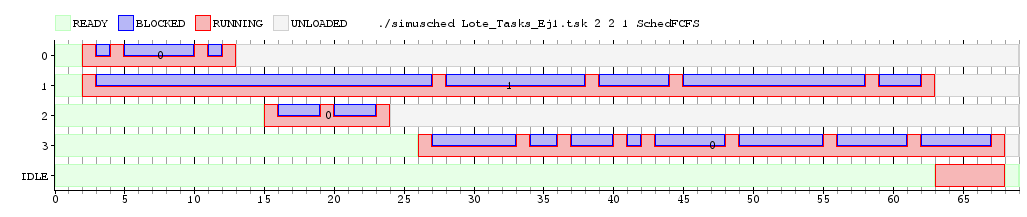
\includegraphics[scale=0.55]{images/Ej1}}
    \caption{FCFS Scheduler con 4 tareas de consola.}
\end{figure}


